\section{Geometric estimates before a change of law}\label{R:geo:section}

This section has two related purposes.  We first derive irreducible
estimates and the laws conditioned on bridge height or on two boundary
ports, using the finite spatial and polygon estimates below together
with renewal factorization.  This route does not use the first-length
estimate or the mass of long bridges from Theorem~\ref{R:renew:finite-input};
it therefore also explains what remains available without those stronger
inputs.

We then estimate the absolute critical mass of unrestricted paths, before
any probability normalization.  Splitting such a path at a turn produces
two bridges that must avoid each other.  We estimate this avoidance under
the independent irreducible law while retaining separate, unused
increments for matching a height or testing a length.  The resulting
turning-chain estimate gives the total-count and rapid-travel bounds used
in the thermal and prescribed-endpoint laws.  Its two-bridge form also
allows arbitrary terminal pieces to be attached without consuming the
height variable needed to compare their final endpoints.

Throughout this section a port path has weight $\rho^L$, where $L$ is its
number of visited vertices.  A port itself has no weight.  Heights are
integers measured in row spacings.  Write $B_h(x)$ for the mass of strict
bridges from a fixed bottom port to displacement $(h,x)$, and
$B_h=\sum_xB_h(x)$.  The horizontal coordinate uses the fixed port lattice;
it may be staggered between successive rows.  For a bridge or an
irreducible, $H$ is its height, $X$ its signed horizontal displacement,
and $D$ its Euclidean diameter.  For a nonnegative function $f$, write
$p(f)=\int f\,dp$; on events $p$ denotes probability.  The law $p$ and the
factorization into independent irreducibles are those of
Proposition~\ref{R:renew:factorization}.  We use $q(t)=p(1-e^{-L/t})$.

\subsection{The finite geometric inputs}\label{R:geo:finite-inputs}

Here are the finite estimates used in this section.  They are the slab,
arch, and polygon theorems of \emph{Radial transfer estimates and polygon
length laws for honeycomb walks}.  We state their full probabilistic
content so that the subsequent changes of law can be read independently
of their analytic proofs~\cite[Theorems~1.1, 12.1, 12.2 and
Proposition~3.1]{companionA}.

\begin{enumerate}
\item For $h\ge1$ and every terminal port,
\begin{equation}\label{R:geo:slab-input}
 c h^{-1/4}\le B_h\le C h^{-1/4},\qquad
 B_h(x)\le C h^{-5/4},\qquad
 B_h[D>Mh]\le C(Mh)^{-1/4}\quad(M\ge1).
\end{equation}
Let $g:[0,1]\to\mathbb R$ be continuous and piecewise linear, with
$g(0)=0$, and fix $\epsilon>0$. The raw bridge mass restricted to
\[
 \{(x,y):0\le y\le h,\ |x-hg(y/h)|\le\epsilon h\}
\]
is at least $c(g,\epsilon)h^{-1/4}$ for all sufficiently large
admissible $h$, in the cut convention of \cite[Theorem~12.2]{companionA}.
The lower port is fixed and the upper port is free. For a compact family
of such graphs in the uniform topology, both the constant and the lower
threshold can be chosen uniformly. In particular this is a
fixed-proportion corridor estimate, without a power loss.
\item The mass $a_b$ of upper-half-plane arches between ports separated
by $b$ along their boundary satisfies $a_b\asymp b^{-5/4}$.  The same
lower bound holds after restricting the diameter to $C b$, for one fixed
$C$.  Also $\sum_{b\ge1}a_b<\infty$.
\item Let $\mathcal P$ be simple unoriented polygons modulo translations,
with weight $w(P)=\rho^{|P|}$.  As $r\to\infty$,
\begin{equation}\label{R:geo:polygon-input}
 \sum_{D(P)\ge r}w(P)=r^{-2+o(1)},\qquad
 \sum_{D(P)\ge r}|P|w(P)=r^{-2/3+o(1)},\qquad
 \sum_{D(P)\le r}|P|^2w(P)\le r^{2/3+o(1)}.
\end{equation}
\item Put $e=(1,0)$ and $a=(1/2,\sqrt3/2)$, and write
$P_{ij}=ie+ja$ and $R_{ij}=P_{ij}+(e+a)/3$ for the two cell types.
Use the same definitions after a lattice symmetry. On the cylinder
obtained by quotienting by $Ne$, count polygons only modulo axial
translation by $a$, and let $S(P)$ be the span of their cell-row indices
$j$. For every fixed $\epsilon>0$, $q\ge0$, and $M>0$,
\begin{equation}\label{R:geo:cylinder-input}
 \sum_{P:S(P)\ge N^{1+\epsilon}}(1+|P|)^q w(P)=O(N^{-M})
\end{equation}
for both contractible and winding polygons. In particular a marked
polygon carries its actual mark multiplicity, which can be absorbed by
the length factor.
\end{enumerate}
The companion locators are Theorem~12.2 for the slab and corridor
estimates, Theorem~12.1 for boundary arches, Theorem~1.1 for the polygon
tails and second moment, and Proposition~3.1 for thin-cylinder span.  Every use below concerns these positive
masses; no conditional mean or prescribed-terminal lower bound is
implicit in \eqref{R:geo:slab-input}.

\subsection{Tails and concentration of an irreducible}

The slab mass determines the height scale of one increment.  Its
pointwise bound and corridor tightness also control horizontal movement.
Both coordinates will be needed when two separately sampled bridges
are joined.

\begin{lemma}\label{R:geo:increment-tails}
There are constants $c,C>0$ such that, for $r\ge1$,
\begin{align}
 p(D>r)&\le Cr^{-3/4},\label{R:geo:D-tail}\\
 p(c r<H<C r)&\ge c r^{-3/4},\label{R:geo:H-shell}\\
 p(c r<|X|<C r,\ H<C r)&\ge c r^{-3/4}.
 \label{R:geo:X-shell}
\end{align}
Consequently, for $Y=H,D$, or $|X|$,
$p(Y\wedge r)\le C r^{1/4}$.  Also
$1-p(e^{-H/r})\asymp r^{-3/4}$.
\end{lemma}
\begin{proof}
Put $\vartheta_r=1-p(e^{-H/r})$.  The renewal identity gives
\[
 \vartheta_r^{-1}=\sum_{h\ge0}e^{-h/r}B_h\asymp r^{3/4}.
\]
After normalization, this bridge sum consists of a geometric number of
increments with one-increment law proportional to $e^{-H/r}p$.
Its number of increments has mean of order $r^{3/4}$.
The inequality $1-e^{-H/r}\ge(1-e^{-1})\mathbf1_{\{H\ge r\}}$
first gives the height tail.

The diameter of the whole bridge divided by $r$ is tight in this
normalized sum, by \eqref{R:geo:slab-input}, summation over heights, and
the exponentially small contribution of heights much larger than $r$.
An increment of diameter greater than $Mr$ forces the same diameter
event for the whole bridge.  The elementary formula for a geometrically
stopped list therefore gives
$p(e^{-H/r};D>Mr)\le C_M\vartheta_r$ for one sufficiently large fixed $M$.
On $H\le r$ the damping is bounded below; the already proved height
tail handles $H>r$.  Rescaling by the fixed $M$ proves
\eqref{R:geo:D-tail}, and integration of that tail proves the truncated
first-moment bounds.

The lower bound for $\vartheta_r$ cannot be supplied by very small or very large
heights.  Indeed their contributions to $p(1-e^{-H/r})$ are at most
$C\delta^{1/4}r^{-3/4}$ for $H\le\delta r$ and
$C M^{-3/4}r^{-3/4}$ for $H>Mr$.  Choosing $\delta$ small and $M$
large proves \eqref{R:geo:H-shell}.

In the normalized bridge sum, heights in $[r,2r]$ have probability
bounded below.  At any such height, the pointwise bound in
\eqref{R:geo:slab-input} shows that terminal positions in an interval
of width $\delta r$ have probability at most $C\delta$.  Thus the
total horizontal displacement has magnitude at least $c r$ with
probability bounded below.  The expected sum of
$\min(|X_i|,\delta r)$ over the geometric list is at most
$C\delta^{1/4}r$; increments of diameter greater than $Mr$ have
arbitrarily small probability when $M$ is large.  Hence, with probability
bounded below, the list contains an increment with
$c' r<|X_i|<C'r$ and $H_i<C'r$.  Its expected number is an upper bound
for that probability.  The geometric mean is of order $r^{3/4}$ and
the tilted probability of this event is at most a constant times its
$p$ probability.  This proves \eqref{R:geo:X-shell}.
\end{proof}
\begin{lemma}[Spatial atoms]\label{R:geo:atoms}
For $k\ge1$, sums of $k$ independent irreducibles satisfy
\[
 \sup_y p^{\otimes k}\{\textstyle\sum_{i=1}^k(H_i,X_i)=y\}
       \le C k^{-8/3},\qquad
 \sup_h p^{\otimes k}\{\textstyle\sum_{i=1}^kH_i=h\}
       \le C k^{-4/3}.
\]
Let $\Gamma$ be the lattice generated by the possible $(H,X)$
increments, and let $\Gamma_1$ be the subgroup generated by their
differences.  On the dual torus of $\Gamma$, the characteristic function
$\varphi$ has modulus one only at the finitely many characters
annihilating $\Gamma_1$.  In a neighborhood of each such character,
\[
       |\varphi(\theta)|\le1-c\,\operatorname{dist}
                  (\theta,\Gamma_1^\perp)^{3/4}.
\]
\end{lemma}
\begin{proof}
Use independent increments $Y,Y'$ in
$1-|\varphi(\theta)|^2=p\otimes p[1-\cos(\theta\cdot(Y-Y'))]$.
Keep $Y'$ in a fixed bounded set of positive probability.  At scale
$r=\epsilon/|\theta|$, Lemma~\ref{R:geo:increment-tails} supplies mass
$c r^{-3/4}$ with the coordinate whose coefficient has larger absolute
value between fixed positive multiples of $r$ in magnitude.  For the
height shell, discard $D>Mr$ with fixed $M$ sufficiently large: the
diameter tail removes at most $CM^{-3/4}r^{-3/4}$, leaving a fixed
fraction of that shell mass.  Both coordinates are now bounded by a
fixed multiple of $r$; the horizontal shell already has this property.
Reflection replaces $X$ by $-X$ without changing $H$.  One of these two
signs avoids cancellation between the two coordinates in the scalar
product.  Choose the fixed $\epsilon>0$ small enough to avoid wrapping
the resulting phase around $2\pi$.  The integrand is then bounded below
by a positive constant on a fixed fraction of this mass.  This gives
the claimed loss near zero.  The same argument using only $H$ proves
the one-dimensional loss.

The support differences span two dimensions: otherwise reflection
would first force an affine relation involving only $H$, and
\eqref{R:geo:H-shell} rules that out.  A finite subset of the differences
therefore generates a rank-two sublattice.  Thus $\Gamma_1$ has finite
index in $\Gamma$.  Equality in the triangle inequality for
$p(e^{i\theta\cdot Y})$ occurs exactly when that character is constant
on the support, which gives precisely the stated finite set.  At each
of these characters its modulus is a translate of the modulus near
zero.  Away from their neighborhoods compactness gives a bound strictly
below one.  Fourier inversion, with
$\int_{\mathbb R^d}e^{-c k|\theta|^{3/4}}d\theta=O(k^{-4d/3})$,
proves both atom estimates.  No span-one assumption in two dimensions
is being made.
\end{proof}

\subsection{Closing two bridges into a polygon}

Let $D_h^*$ be the mass of ordered disjoint pairs of bridges from two
fixed adjacent bottom ports to arbitrary ordered distinct top ports at
height $h$.  Let $D_h$ be its restriction to adjacent top ports,
summed over their common translate.  These are pair masses, rather than
probability laws.

\begin{lemma}\label{R:geo:polygon-sewing}
For each fixed $C$, as $r\to\infty$,
\begin{align}
 \sum_{r\le h\le2r}D_h^*[D(\gamma_1\cup\gamma_2)\le Cr]
       &\le r^{-1/4+o(1)},\label{R:geo:pair-sewing}\\
 \sum_{r\le h\le2r}B_h[L;D\le Cr]
       &\le r^{25/12+o(1)}.\label{R:geo:length-sewing}
\end{align}
In particular
\begin{equation}\label{R:geo:truncated-reward}
 p(L;D\le r)\le r^{7/12+o(1)},\qquad
 q(t)\le t^{-9/16+o(1)}.
\end{equation}
\end{lemma}
\begin{proof}
For a polygon of diameter in $[c r,C'r]$, let $K$ count horizontal row
cuts crossed exactly twice.  Mark $s$ of these cuts, allowing repeated
marks, and order their distinct levels.  Outside the extreme cuts
there are two arches.  Between successive cuts there are two bridges.
Anchor the first cut and its left crossing port, sum its arch gap using
$\sum_b a_b<\infty$, and drop all further disjointness restrictions.
Each internal gap contributes at most
$\sum_{t\le C''r}B_t^2\le C\sqrt r$.  Repeated marks and the choices
of the extreme cuts contribute a fixed polynomial in $r$ whose degree
does not depend on $s$.  Consequently
\[
       \sum_{D(P)\le C'r}w(P)K(P)^s\le C_s r^{C_0+s/2}.
\]
Apply H\"older with arbitrarily large fixed $s$ and the first two
bounds in \eqref{R:geo:polygon-input}.  For the length-weighted measure
use also $|P|\le C r^2$ in the high-moment bound.  We obtain
\[
 \sum_{c r\le D(P)\le C'r}w(P)K(P)\le r^{-3/2+o(1)},\qquad
 \sum_{c r\le D(P)\le C'r}|P|w(P)K(P)^2\le r^{1/3+o(1)}.
\]

Close a pair counted by $D_h^*$ with a fixed bounded lower cap and an
independent upper arch.  The latter has mass at least $c r^{-5/4}$
and diameter at most $C'r$; the two exterior half-planes keep the
closures disjoint from the bridges.  The lower cut is at bounded
distance from the bottom of the resulting polygon.  An output polygon
has at most $C K$ preimages, since choosing its upper cut recovers both
bridges and both caps.  This proves \eqref{R:geo:pair-sewing}.

For \eqref{R:geo:length-sewing}, place a second bridge in a disjoint
box to the right.  Its starting port has order $r$ choices and its
confined mass is at least $c r^{-1/4}$.  Close with exterior arches
above and below, each of mass at least $c r^{-5/4}$.  The added mass
per input is at least $c r^{-7/4}$.  Both separating cuts recover the
construction with multiplicity at most $C K^2$, and the input length
is bounded by the output polygon length.  The preceding weighted
bound gives $r^{7/4+1/3+o(1)}=r^{25/12+o(1)}$.

Finally surround an irreducible of diameter at most $r$ by confined
bridges whose heights each range over $[r,2r]$.  Each side has mass at
least $c r^{3/4}$.  In the output bridge the sum of the lengths of all
possible marked irreducibles is at most its full length.  Applying
\eqref{R:geo:length-sewing} on a bounded number of height bins therefore
gives $p(L;D\le r)\le r^{25/12-3/2+o(1)}$.  In
$q(t)\le t^{-1}p(L;D\le r)+p(D>r)$ take $r=t^{3/4}$.
\end{proof}

\subsection{Avoidance of adjacent initial pieces}

Two independent increment lists begun at adjacent ports need not stay
disjoint.  Define $E_k$ to be the event that their first $k$ increments
can be extended to two disjoint bridges ending at one common height,
while remaining their initial $k$ renewal pieces.  Equivalently the
extensions are strict bridges above the terminal renewal cuts.
This event concerns the finite prefixes; those extensions need not be
the independently sampled continuations.

\begin{lemma}\label{R:geo:fence}
For each $\delta>0$ there is $C_\delta$ such that
$p^{\otimes\mathbb N}\otimes p^{\otimes\mathbb N}(E_k)
\le C_\delta(1+k)^{-1+\delta}$.
\end{lemma}
\begin{proof}
We prove this bound by induction, for $0<\delta<1$.  Set $r=k^{4/3}$
and expose $k_0=\lfloor k/2\rfloor$ increments on each side.  Call
their endpoint coordinates $(X_i,t_i)$.  If the sum of their diameters
exceeds $Mr$, the sum of the diameters truncated at $Mr$ also does.
On $E_k$ every earlier paired prefix satisfies $E_{a-1}$.  Markov's
inequality and independence of the next increment give an upper bound
\[
 \frac1{Mr}\sum_{i=1}^2\sum_{a\le k_0}
       \Pr(E_{a-1})p(D\wedge Mr)
 \le C_\delta M^{-3/4} A_\delta k^{-1+\delta},
\]
where $A_\delta$ is the induction constant.  Choose $M$ large enough
that this is at most one quarter of the proposed bound.

Label the lower endpoint path 1, so $t_1\le t_2$, and reflect
horizontally if necessary so that it starts at the left port.  For
small fixed $d>0$, let $m$ be the leftmost coordinate of the second
history between heights $t_1$ and $t_1+dr$, with $m=+\infty$ if it
has no point there.  We discard $|m-X_1|\le ur$, where $u>0$ will
be small.  Condition on both histories through $\lfloor k/4\rfloor$
increments and then on the rest of the second history.  For each
possible $t_1=O(Mr)$, the prohibited interval for $X_1$ has width
$2ur+O(1)$.  The two-dimensional atom bound on the still independent
part of the first history shows that this conditional probability is
at most $C_M(u+r^{-1})$.  The induction bound for
$E_{\lfloor k/4\rfloor}$ pays for the earlier histories.

Next discard the case $m<X_1-ur$.  Were a disjoint common-height
extension possible, the left crosscut would separate the second path
from the far left of the slab.  Thus its continuation above $t_1$
would have to pass to the left of a point of the second history in
this band; at height $t_1$ such a point is already excluded by the
single crossing there.  In the next $\lfloor sk\rfloor$ increments,
however, the first path, with probability as close to one as desired,
gains height greater than $dr$ while its total diameter sum is less
than $ur$.  Indeed the latter exceptional probability is at most
$C s u^{-3/4}$ by truncation and the diameter tail.  The probability
of no height increment exceeding $dr$ is at most
$\exp(-c s d^{-3/4})$, by the height shell lower bound.  Choose $s$
small after $u$, and $d$ small after $s$.  These fresh increments
fit among the first $k$ and are independent of the exposed histories.
They contradict the required leftward passage.  Conditional on those
histories their failure probability is uniformly small.  The induction
bound at $\lfloor k/4\rfloor$, with $u,s,d$ chosen in that order,
makes the total of these two discarded cases, including reflected
cases, at most another quarter of $A_\delta k^{-1+\delta}$.

For each remaining pair of histories the strip just above $t_1$ of
height $dr$, to the left of $X_1+ur$, is free of the second history.
Extend the first history through this strip to the left of the box
containing both histories, then upward.  Extend the second upward in
a separate corridor.  If $t_2<t_1+dr$, its tip lies to the right of
the cleared strip; if $t_2\ge t_1+dr$, the first path has reached
its separate corridor before the second extension begins.  These are
piecewise linear guides with fixed positive separation.  The corridor
input supplies joint mass at least $c r^{-1/2}$ to every common
terminal level in $[C_Mr,2C_Mr]$.  The diameter stays at most $C'_Mr$.

In an output pair the original histories are recovered by cutting
after exactly $k_0$ irreducibles on both paths.  Hence there is no
multiplicity factor for those cuts.  Summing the order $r$ terminal
levels and using \eqref{R:geo:pair-sewing}, the mass of the remaining
histories is at most $r^{-3/4+o(1)}=k^{-1+o(1)}$.  For large $k$
this fits in the remaining half of the induction bound.  Increasing
$A_\delta$ handles the finitely many smaller $k$.
\end{proof}

\subsection{Matching the two ends of a marked pair}
\label{R:geo:matching-section}

The previous lemma controls initial avoidance.  The next estimate also
pays for matching the far endpoints.  Its mark may be any nonnegative
function of one whole irreducible; this uniformity is what permits both
length and diameter tests later.

\begin{proposition}\label{R:geo:marked-pair}
For every nonnegative function $f$ of an irreducible, with $p(f)<\infty$,
and every $\epsilon>0$,
\begin{equation}\label{R:geo:marked-pair-bound}
 \sum_{R\le h\le2R}D_h\left[\sum_{i\text{ in the first path}}f(I_i)\right]
       \le C_\epsilon R^{-5/4+\epsilon}p(f).
\end{equation}
Either path can carry the mark.  If the two bottom ports instead have
any prescribed separation, while the top ports remain adjacent, the
right side becomes $C_\epsilon R^{-1/2+\epsilon}p(f)$.  In that second
estimate, requiring the marked path to contain at most
$R^{3/4-\delta}$ increments improves the bound by
$R^{-\delta+\epsilon}$, with the exponent slacks combined in the
constant.
\end{proposition}
\begin{proof}
Fix a small $\eta>0$.  Lists with more than $R^{3/4+\eta}$ increments
have superpolynomially small mass: after removing the marked slot,
exponential Markov with $e^{-H/R}$ gives $\exp(-cR^\eta)$.
There are at most $2R$ increments on either list, so summing all counts
and possible marks still bounds this part by $p(f)R^{-M}$ for any
fixed $M$.  We henceforth impose the count cutoff.

Bin the numbers of increments before and after the marked slot on the
first path, each increased by one, at dyadic scales $a_-,a_+$.
There are $O(a_-a_+)$ choices of these two numbers.  Fix them, and put
$K=\max(a_-,a_+)$.  Near each end of the second path choose a grid
of more than $2/\eta$ height thresholds in a fixed small fraction of
$R$.  The counts to their first reaching renewals are positive and at
most $2R$.  At some consecutive pair the counts differ by a factor at
most $R^\eta$.  Bin the lower count at scale $c_e$, where $e=-,+$
specifies the end.  Sum over these finitely many threshold choices and
logarithmically many bins at the end.

At each end expose $m_e=\lfloor R^{-2\eta}\min(a_e,c_e)\rfloor$
increments on both paths.  If necessary reduce this by a fixed factor
to account for the added one in $a_e$; zero histories cost one.  For
large $R$ these are disjoint coordinate blocks and do not include the
mark.  On the second path they lie before the selected lower height
thresholds.  On the first path that extra restriction is unnecessary:
the actual full disjoint bridges supply the extensions required by
the prefix event.  At the
upper end read the lists backwards in relative coordinates from
adjacent ports.  Their still unknown common translation is immaterial
to this test.  Lemma~\ref{R:geo:fence} supplies the independent cost
\begin{equation}\label{R:geo:end-costs}
 R^{O(\eta)}\prod_{e=-,+}\min(a_e,c_e)^{-1}.
\end{equation}

The choices of counts and of the marked slot cost $O(a_-a_+)$.  To
cancel that cost against the two history factors, we will obtain a
matching gain $\min(1,c_e/K)$ at each end.  We first bound the central
part of the second path, then match its displacement using an independent
batch of increments on the first path.

Fix the histories.  Sum over the remaining count on the second path
and let $F(y)$ be its central bridge kernel, where $y$ is its two-dimensional
displacement.  Its height is comparable to $R$.  From either end,
within $O(c_eR^\eta)$ central increments it must gain at least
$c_\eta R$ height, by the gap between the two selected thresholds.
Retain these requirements and drop the other restrictions.  The
pointwise slab estimate gives $F(y)\le CR^{-5/4}$.

We need the following improvement on a small displacement ball $U_b$,
valid for $1\ll b\ll c_\eta R$ and either subset $S$ of the two ends:
\begin{equation}\label{R:geo:central-kernel}
 \sum_{y\in U_b}F(y)\le CR^{-5/4}b^2
           \prod_{e\in S}(C_\eta c_eR^\eta b^{-3/4}).
\end{equation}
To prove it, append at each indicated end an independently chosen
bridge of height in $[b,2b]$ and diameter at most $Cb$.
Its mass, with terminal position and height summed, is at least
$c b^{3/4}$.  The enlarged displacement lies in a ball of radius
$C'b$, hence has at most $Cb^2$ possible values, each with mass
$CR^{-5/4}$.  In any output, a possible removed attachment ends
within $O(b)$ height of the new endpoint.  Moreover that cut precedes
the first renewal at or beyond height $c_\eta R/2$ from the new endpoint by at most
$O(c_eR^\eta)$ renewal steps.  Thus there are at most that many
possible cuts at each indicated end.  Dividing by the attachment
masses proves \eqref{R:geo:central-kernel}.  Positivity is used both
in adjoining these bridges and in dropping all further restrictions.

The first path still has order $K$ unexposed increments outside the
mark and the histories.  If $K\le R^{5\eta}$, the pointwise bound
on $F$ suffices, since all additional factors below cost only
$R^{O(\eta)}$.  Otherwise choose
$b_0=\lfloor KR^{-4\eta}\rfloor$ slots in each of
$\lceil30/\eta\rceil$ disjoint batches.  Put
$b=R^\eta b_0^{4/3}$.  The count cutoff implies
$b\le R^{1-3\eta}$, up to fixed factors.  By the diameter tail and
truncation, a batch has displacement norm greater than $b$ with
probability at most $C R^{-3\eta/4}$.  The batches are independent,
so the chance that all of them fail is $O(R^{-10})$.

On that exception use the pointwise bound on $F$.  Otherwise take a
union over the fixed finite set of possible successful batch labels.
For each label, fix everything outside that batch and use its
two-dimensional atom bound $C b_0^{-8/3}$ together with
\eqref{R:geo:central-kernel}.  At the end $e$ use the improvement
when $c_e<K$.  Since $b_0^{-8/3}b^2=R^{2\eta}$ and
$c_eR^\eta b^{-3/4}\le R^{O(\eta)}c_e/K$, the resulting matching
cost is
\begin{equation}\label{R:geo:matching-cost}
 C_\eta R^{-5/4+O(\eta)}
                  \prod_{e=-,+}\min(1,c_e/K).
\end{equation}
The estimate is uniform in the value of the marked increment.
The mark can therefore be integrated separately at cost $p(f)$.

Multiply \eqref{R:geo:matching-cost} by \eqref{R:geo:end-costs}
and the $O(a_-a_+)$ count and mark choices.  Each end contributes at
most one because
\[
       a_e\min(1,c_e/K)\le\min(a_e,c_e).
\]
Summing the threshold and dyadic labels costs only logarithmic powers.
Taking $\eta$ sufficiently small in terms of $\epsilon$ proves
\eqref{R:geo:marked-pair-bound}.

For prescribed separated bottom ports, retain exactly the same central
kernel and matching proof.  The displacement to be matched is merely
shifted by that prescribed separation.  The bottom avoidance test is
now absent, so its factor in \eqref{R:geo:end-costs} is lost.  The
remaining count factor is bounded by
\[
 \frac{a_-a_+\prod_e\min(1,c_e/K)}{\min(a_+,c_+)}
       \le a_-\le R^{3/4+\eta}.
\]
This proves the $R^{3/4+\epsilon}$ loss.  If the marked path has at
most $R^{3/4-\delta}$ increments, then $a_-\le C R^{3/4-\delta}$,
which gives the stated improvement.  This is the only change in the
argument; no bottom avoidance probability is retained implicitly.
\end{proof}

The next consequence recovers the length-deficit exponent from the
spatial and polygon inputs alone.  Proposition~\ref{R:renew:increments}
gave the stronger bounded-factor estimate using the finite first-length
and long-bridge estimates.
\begin{corollary}\label{R:geo:deficit}
The length deficit satisfies $q(t)=t^{-9/16+o(1)}$.
\end{corollary}
\begin{proof}
The upper bound is \eqref{R:geo:truncated-reward}.  For a lower bound
fix $\eta>0$.  On polygon diameters in $[r,r^{1+\eta}]$, the
length-weighted mass is $r^{-2/3+o(1)}$.  Lengths less than
$r^{4/3-\eta}$ contribute at most $r^{-2/3-\eta+o(1)}$ by the
unweighted tail.  Lengths greater than $r^{4/3+2\eta}$ contribute
at most
\[
 r^{-4/3-2\eta}\sum_{D(P)\le r^{1+\eta}}|P|^2w(P)
       \le r^{-2/3-4\eta/3+o(1)}.
\]
Thus the unweighted mass with both diameter and length in these
windows is at least $r^{-2-2\eta+o(1)}$.

Choose a symmetry-related row normal retaining a fixed fraction with
vertical span comparable to diameter.  A bounded hexagonal-face
modification at its lowest and highest vertices turns the polygon
into two disjoint bridges with adjacent ports at each end.  Here is
the local operation.  In coordinates
$P_{ij}=iu+jv$, $R_{ij}=P_{ij}+(u+v)/3$, with
$u=(1,0)$ and $v=(1/2,\sqrt3/2)$, the neighbors of $P_{ij}$ are
$R_{ij},R_{i-1,j},R_{i,j-1}$.  A lowest polygon vertex is a $P$
and uses both ascending bonds.  At the leftmost lowest such vertex,
take the adjacent face below and to its right.  Its overlap with the
polygon is a path of one or two edges and includes every occupied
vertex of that face.  Symmetric difference replaces it by the
complementary face path, creating a bounded exterior lower cap.
The reflected operation creates the upper cap.  Remove the two caps.
Simplicity forces the remainder to be exactly two through bridges;
otherwise one cap would bound a separate cycle.  The faces are
disjoint for large $r$, and length, diameter, and weight change by
bounded amounts.  Anchoring the lower left port, the cuts and caps
recover the input with bounded multiplicity.  This suffices for the
mass lower bound, whether or not a tie convention makes the map
injective.

The output heights lie between $cr$ and $Cr^{1+\eta}$.  Set
$t=r^{4/3-2\eta}$.  Across both output lists,
$\sum_i(1-e^{-L_i/t})\ge1-e^{-\sum_iL_i/t}$ is bounded below by a
positive constant.  Apply Proposition~\ref{R:geo:marked-pair} with
$f=1-e^{-L/t}$ to both paths and sum the height bins.  It gives
$r^{-2-2\eta+o(1)}\le r^{-5/4+o(1)}q(t)$, hence
$q(t)\ge r^{-3/4-2\eta+o(1)}$.  Letting $\eta$ decrease proves
the lower exponent.
\end{proof}

\subsection{Height conditioning and fixed boundary ports}

These two applications keep their distinct normalizing masses.  A
bridge with terminal port summed has mass $h^{-1/4}$; an arch with
both boundary ports prescribed has mass $r^{-5/4}$.  The missing
bottom avoidance test in Proposition~\ref{R:geo:marked-pair} is
exactly what changes the accounting between them.

\begin{proposition}\label{R:geo:fixed-height}
Under the critical law on strict bridges of height $h$, with terminal
port unrestricted, $L=h^{4/3+o(1)}$ and $D=h^{1+o(1)}$ in probability.
The same holds after any restriction retaining a fixed positive
fraction of $B_h$.
\end{proposition}
\begin{proof}
For counts in $[k,2k)$, split each list into two groups of comparable
size.  If their total height is $h$, one group gains at least $h/2$,
at cost $C\min(1,k h^{-3/4})$; the other matches the remaining
height at cost $C(1+k)^{-4/3}$.  There are $O(k)$ count choices.
Thus counts at most $h^{3/4-\delta}$ have total mass at most
$h^{-1/4-2\delta/3+o(1)}$, negligible compared with $B_h$.
Bounded counts follow directly from the height tail.  Counts exceeding
$h^{3/4+\delta}$ have superpolynomially small mass by exponential
Markov with $e^{-H/h}$.

On the remaining counts, length at most $t=h^{4/3-\epsilon}$ costs
at most $e\exp(-k q(t))$.  Choose $\delta<9\epsilon/32$; the
deficit estimate makes this superpolynomially small.  For length
greater than $t=h^{4/3+\epsilon}$, mark
$1-e^{-L_i/t}$, whose sum is bounded below on that event.  The other
increments match height at cost $Ck^{-4/3}$.  Summing marks and count
choices gives $Ck^{2/3}q(t)$ in a dyadic bin.  For sufficiently small
$\delta$ this is $o(h^{-1/4})$.  Finally $D\ge c h$
deterministically, and \eqref{R:geo:slab-input} gives
$B_h[D>h^{1+\epsilon}]=o(B_h)$.  Division by any retained fixed
fraction of $B_h$ preserves every conclusion.
\end{proof}

\begin{proposition}\label{R:geo:arch-law}
For the critical upper-half-plane law between two prescribed boundary
ports at separation $r$, one has $L=r^{4/3+o(1)}$ and
$D=r^{1+o(1)}$ in probability.  Any restriction retaining a fixed
positive fraction of the arch mass has the same exponents.
\end{proposition}
\begin{proof}
The denominator is $a_r\asymp r^{-5/4}$.  First discard arches of
height at most $r^{1-\epsilon}$.  Glue two independent such arches,
one reflected into the lower half-plane, to make a marked polygon.
This squares their total mass, up to bounded weight factors.  Choose
a symmetry-related period of order $r^{1-\epsilon}$ whose vertical
component exceeds the polygon's span.  Its projection is simple,
and anchoring the first marked edge recovers the lift.  The transverse
span is of order at least $r$, because of the original boundary gap
and the nonparallel period.  The possible marks cost at most a length
factor.  The cylinder estimate \eqref{R:geo:cylinder-input}, with
arbitrarily large $M$, makes the squared mass and hence the mass
itself smaller than every power of $r$.

For every remaining arch perform only the upper extremal-face
operation described in the proof of Corollary~\ref{R:geo:deficit}.
Removing the new upper cap leaves two disjoint bridges from the
original prescribed bottom ports to adjacent top ports.  Weights and
lengths change boundedly and the inverse multiplicity is bounded.
At height $h\in[R,2R]$, Proposition~\ref{R:geo:marked-pair} with
the bottom test omitted gives
$R^{-1/2+o(1)}p(f)$ for a mark on either path.  Take
$f=\min(1,H/R)$: its sum on either path is bounded below, while
$p(f)\le CR^{-3/4}$.  The total mass of the bin is therefore
$R^{-5/4+o(1)}$.  Summing $R>r^{1+\epsilon}$ is negligible relative
to $a_r$.

In the remaining height range $[r^{1-\epsilon},r^{1+\epsilon}]$,
requiring one path to have count at most $R^{3/4-\delta}$ adds the
factor $R^{-\delta+o(1)}$.  Choose $\epsilon$ small after $\delta$;
these pairs are negligible.  For larger counts, a total length at
most $r^{4/3-\delta'}$ is superpolynomially unlikely under the free
increment law, by $\exp(-k q(r^{4/3-\delta'}))$.  One may drop
all pair constraints here; each count is at most $2R$, so their
choices cost only a polynomial.  Taking $\epsilon,\delta$ small
enough in terms of $\delta'$ proves the lower length bound.

For the upper length bound mark $f=1-e^{-L/t}$ with
$t=r^{4/3+\delta'}$.  Summing the two paths in the typical height
bins gives $R^{-1/2+o(1)}q(t)$, which is $o(r^{-5/4})$ when
$\epsilon$ is sufficiently small.  For diameter greater than
$r^{1+\delta'}$, use instead $f=\min(1,D/r^{1+\delta'})$.
The sum of increment diameters dominates each path diameter, and
Lemma~\ref{R:geo:increment-tails} bounds its expectation by
$Cr^{-3(1+\delta')/4}$.  The same calculation applies.  The lower
diameter bound follows from the prescribed boundary gap.  Bounded
offsets in the cap construction are absorbed by decreasing exponent
slacks.  A retained positive fraction of the denominator changes
none of the estimates.
\end{proof}
\subsection{A joint estimate for turning chains}

We now estimate path pieces before choosing any probability normalization.
A \emph{turn} joins two consecutive pieces that both run away from their
joining vertex toward the same side in height.  We first convert these
pieces into strict port bridges, then integrate their irreducible
coordinates while retaining the necessary avoidance tests.

\begin{lemma}[Converting endpoints to ports]\label{R:geo:port-repair}
Suppose a simple path segment stays between the heights of its endpoints.
If its span is sufficiently large, bounded endpoint changes convert it
into a strict port bridge.  At a turn between two such segments, the
changes can be made jointly so that their ports are adjacent and their
initial parts remain disjoint through a fixed positive fraction of the
smaller span.  Changes at opposite ends of a large-span segment occur in
disjoint height zones.

The original ordered segments, with one initial anchor, can be recovered
from the resulting ordered bridges and at most constantly many local
choices per segment.  Lengths and endpoint heights change by bounded
amounts per end.  Bounded-span segments can instead be represented by
positive-height bridges and a class of one-row paths with bounded total
critical mass and an exponential length tail.
\end{lemma}
\begin{proof}
Use the $P,R$ coordinates in the proof of
Corollary~\ref{R:geo:deficit}.  At a top endpoint an $R$ extends by its
upward bond to the next cut; a top $P$ must have been reached along its
unique descending bond and can be trimmed to the port immediately below.
No other top $P$ is internal to the segment, since it has only one
descending bond.  Reflect at bottom endpoints.

At a common top turn the pivot is an $R_{ij}$ using both descending bonds.
Use the face immediately above and to its right, with lower path
$R_{ij},P_{i+1,j},R_{i+1,j}$.  If the other uppermost $R_{i+1,j}$ is
occupied, it too uses both descending bonds.  The union's overlap with
this face is therefore a path of one or two edges containing all its
occupied face vertices.  Symmetric difference with the face, followed by
removal of the new upper cap, creates disjoint ends at adjacent ports.
Reflect at a bottom turn.  Only boundedly many bonds change.  For large
spans the far-end modification cannot affect disjointness within, say,
one quarter of the smaller original span from this turn.

If individual trimming makes the endpoint levels meet or cross, the
segment was confined to one row.  Its induced graph has degree at most
two, so there are at most constantly many paths of each length from its
endpoint.  Their critical weights have an exponential tail because
$\rho<1$.  Otherwise the result is a positive-height bridge.  Record the
case, each bounded local change, and the offsets between consecutive
ports.  There are constantly many such records per piece, and reversing
them recovers the original path.  The next anchor is determined by the
preceding piece and its record; no free translation factor is added.
\end{proof}

Consider a chain of $m$ bridge nodes, each with at most two tested ends.
A tested turn requires the corresponding prefixes, read in the same
upward direction, to be disjoint for a fixed positive fraction of the
smaller height.  Fix their local records.  At node $i$, restrict height
to $[cR_i,CR_i]$ and irreducible count to $[k_i,2k_i)$, with fixed
$c,C>0$.  All scales and counts are at most $C_0h$.  Put
\[
 K_i=R_i^{3/4},\qquad \kappa_i=\min(k_i,K_i),\qquad
 s_{ij}=\min(\kappa_i,\kappa_j).
\]
The scales $R_i$ need not be comparable between different nodes.

\begin{proposition}[Independent coordinates at a turn]
\label{R:geo:chain}
For every sufficiently small fixed $\eta>0$, the joint critical mass,
including all actual count choices in the bins, is at most
\begin{equation}\label{R:geo:chain-product}
 h^{C_1\eta(m+1)}\prod_i\frac{\kappa_i^2}{K_i}
                    \prod_{ij\text{ tested}}s_{ij}^{-1}
\end{equation}
for $h$ sufficiently large depending on $\eta$.  Constant factors per
node are included in this bound.

At each sufficiently large-count node, the proof leaves an independent
group of at least $c k_i$ increments available for a concentration test.
An interval of at most $a_i$ allowed total heights contributes
\begin{equation}\label{R:geo:height-factor}
                    C\min(1,a_i\kappa_i^{-4/3}),
\end{equation}
provided the interval is measurable outside that group, with any fixed
external data allowed.  A proved concentration bound for another
additive statistic, such as length, may be used on this group instead.
A different independent group supplies
\begin{equation}\label{R:geo:short-factor}
                         C e^{-c k_i q(l)}
\end{equation}
when the node's total length is at most $l$.

Several height factors may be used for a specified vector of heights and
then summed over an explicitly bounded admissible set, or in a successive
integration order with the stated measurability property.  The estimate
does not condition on the reserved group's own horizontal displacement.
Bounded-count nodes have the trivial bounded-factor version of the height
estimate.  One-row paths have $K_i=\kappa_i=1$ and bounded mass, with no
atom or independent length test asserted.
\end{proposition}
\begin{proof}
Fix every actual count.  At $e=ij$ put $d_e=\min(R_i,R_j)$ and
$s_e=s_{ij}$.  If $d_e$ is bounded in terms of $\eta$, drop this test
at a bounded cost.  Otherwise place more than $3/\eta$ consecutive
thresholds within a small fixed fraction of $d_e$ from each incident
end, with gaps at least $c_\eta d_e$.  The counts to their first
reaching renewals lie in $[1,C_0h]$.  At some consecutive pair their
ratio is at most $h^\eta$, since otherwise their product would exceed
the count cap.  Bin the lower crossing counts dyadically at $c_{i,e}$
and $c_{j,e}$, and put $c_e=\min(c_{i,e},c_{j,e})$.

Once these labels are fixed, the first
$\ell_e=\lfloor h^{-2\eta}c_e\rfloor$ slots at both ends are
deterministic coordinate sets.  On the actual event their heights are
below the lower thresholds, and the actual disjoint paths extend them
to a common cut within the tested range.  Opposite-end histories are
disjoint coordinate blocks: each uses a vanishing fraction of the
node's count.  Lemma~\ref{R:geo:fence} supplies the independent cost
\begin{equation}\label{R:geo:history-charge}
                        C_\eta h^{3\eta}/c_e.
\end{equation}
This includes $\ell_e=0$.  If $c_e\ge h^{-4\eta}s_e$, it already
costs at most $C_\eta h^{7\eta}/s_e$.

If $c_e<h^{-4\eta}s_e$, designate an incident node attaining this
smaller bin.  On it take the deterministic group of slots
\[
                    \ell_e+1,\ldots,\lceil2h^\eta c_e\rceil
\]
read from that end.  It contains the later threshold renewal, so its
height sum is at least $c_\eta d_e$.  It has at most
$C c_eh^\eta\le C h^{-3\eta}s_e\le C h^{-3\eta}k_i$ slots.
Call it a rapid group.  Such groups are disjoint from the histories and
from any opposite-end rapid group.  The height tail and its truncated
first moment imply
\begin{equation}\label{R:geo:sum-tail}
 \Pr(H_1+\cdots+H_n\ge u)\le C\min(1,n u^{-3/4}).
\end{equation}
The rapid group therefore costs at most
$C_\eta c_eh^\eta/d_e^{3/4}\le C_\eta h^\eta c_e/s_e$.
Multiplying by \eqref{R:geo:history-charge} pays $s_e^{-1}$.
We now discard the original crossing-index restrictions: only necessary
events on the deterministic independent coordinate blocks are retained.

The histories removed at one node have total height less than a small
fixed multiple of $R_i$.  Their complement must gain at least $c_0R_i$.
It consists of at most two rapid groups and the remaining slots.
Partition those remaining slots into eight groups of nearly equal size.
For sufficiently large fixed counts, each has order $k_i$ slots.
Some one of these at most ten groups gains height at least $c'_0R_i$.
Take a finite union over a label selecting that height-carrying group.
\emph{After} fixing the label, reserve three different free groups for
count damping, concentration, and the length test.  None is the
height-carrying group.

Write $b_i=\min(1,k_i/K_i)$.  If a free group carries the height,
\eqref{R:geo:sum-tail} charges it by $Cb_i$, independently of the
rapid groups.  If the carrier is the rapid group for $e$ on node $i$,
charge its larger height directly at scale $R_i$.  The cost
$C_\eta c_eh^\eta/K_i$ supplies both required factors, because
\begin{equation}\label{R:geo:shared-height-charge}
              c_e/K_i\le \min(1,k_i/K_i)c_e/s_e.
\end{equation}
This follows from $s_e\le\kappa_i$ in either regime for $k_i/K_i$.
The other rapid group, if any, remains independent.  Also
$d_e^{3/4}=\min(K_i,K_j)\ge s_e$; thus this calculation allows
unrelated height scales.

The reserved damping group has height at most $CR_i$.  Exponential
Markov and $1-p(e^{-H/R_i})\ge c/K_i$ give
$C e^{-c k_i/K_i}$.  All previously charged events use other slots.
Conditional on coordinates outside the concentration group, its product
law is unchanged.  Lemma~\ref{R:geo:atoms} bounds its height atom by
$Ck_i^{-4/3}\le C\kappa_i^{-4/3}$, proving
\eqref{R:geo:height-factor}.  The same statement holds with any proved
concentration function for an additive statistic of these slots.  On
the separate length group,
\[
 \Pr\{\textstyle\sum L_j\le l\}
       \le e(1-q(l))^{c k_i}\le C e^{-c k_i q(l)}.
\]
These bounds multiply because their coordinate sets are disjoint.
For several height constraints, condition outside all their groups,
bound the joint atom by the product, and sum the allowed height vectors.
Successive interval constraints follow by successive integration with
the same uniform bounds.

For bounded counts the incident turn factors are bounded.  Drop them
and apply \eqref{R:geo:sum-tail} to the whole list.  The height factor
is then bounded below by a positive constant, so its insertion changes
only the constant; no large-count length test is needed.
There are $O(k_i)$ actual counts at each node, and
\[
 k_i\min(1,k_i/K_i)e^{-c k_i/K_i}\le C\kappa_i^2/K_i.
\]
For $k_i\le K_i$ this is immediate; otherwise use $x e^{-cx}\le C$.
Thresholds, crossing-count bins, height-carrier labels, and local records
number at most $(C_\eta\log^C h)^{C(m+1)}$.  These choices and the
power losses above are at most $h^{C_1\eta(m+1)}$ for large $h$.
This proves the proposition.
\end{proof}

\begin{corollary}[Two ends with a reserved height variable]
\label{R:geo:two-ends}
Suppose two bridges start at adjacent prescribed ports and stay disjoint
through a fixed positive fraction of the smaller height.  Their heights
and counts lie in the independent bins above, all bounded by $CN^2$.
For every $\epsilon>0$ their critical mass is at most
\begin{equation}\label{R:geo:two-end-mass}
 C_\epsilon N^\epsilon F,\qquad
 F=\frac{\kappa_1^2\kappa_2^2}
              {K_1K_2\min(\kappa_1,\kappa_2)}.
\end{equation}
An interval of $C(1+r)$ allowed heights on node $i$, measurable outside
its reserved group, adds $\min(1,(1+r)\kappa_i^{-4/3})$.
In particular this applies to the difference of the final endpoint
heights after any two terminal pieces have been fixed up to translation.
For one nonempty bridge the factor is $\kappa_i^2/K_i$, with the same
optional concentration test.
\end{corollary}
\begin{proof}
Take $h=C'N^2$ in Proposition~\ref{R:geo:chain} and choose $\eta$
sufficiently small in terms of $\epsilon$.  Once terminal pieces and
local records are fixed, their final-height constraint reads
$H_i\in[H_j+b-r-C_0,H_j+b+r+C_0]$.  The interval depends on the other
bridge and fixed external data, hence is measurable outside the selected
group.  No horizontal displacement of that group has been fixed.
The one-node assertion is the proposition with no turn test.
\end{proof}

\subsection{Absolute critical mass of unrestricted paths}

The preceding estimate pays for every turn in a chain.  Many turns
therefore make an ordered extremum decomposition inexpensive, even though
we impose no length damping.  This is the point at which the
bridge-unfolding method of Hammersley and Welsh is useful
\cite{HammersleyWelsh1962,MadrasSlade1993}.

\begin{proposition}\label{R:geo:absolute-count}
Let $a_n$ be the total critical mass of plane walks with $n$ visited
vertices, rooted at one specified vertex, or counted up to translations
with both possible initial vertex types.  For every $\delta>0$,
\[
                         a_n\le C_\delta e^{n^\delta}.
\]
The same bound holds for the mass with length at most $n$.  In the
extremum decomposition below, a bounded number of specified pieces may
be omitted and counted separately; all other pieces still cost at most
$C_\delta e^{n^\delta}$, including their count, position, and local
records.
\end{proposition}
\begin{proof}
Split a path at a global minimum of its height and read both parts
outward from that minimum.  In either part, end the first piece at the
last maximum of the remaining path, the next at its last minimum, and
continue.  Each piece stays between its endpoint heights.  The spans
decrease strictly after a possible initial equality, since the selected
extreme cannot occur again in the remaining path.  Every honeycomb edge
has nonzero vertical projection in these coordinates.

In a dyadic span bin $[R,2R)$ there are at most $CR$ pieces in a chain.
Convert their endpoints by Lemma~\ref{R:geo:port-repair}.  Test turns
only between consecutive pieces in the same bin.  An omitted piece
splits that bin into runs; no test crosses an omission.  At a run of
$m$ pieces put $K=R^{3/4}$ and $x_i=\kappa_i/K\le1$, absorbing
fixed comparability constants into the per-node constants.  The product
in \eqref{R:geo:chain-product}, before its exponent loss, is
\begin{equation}\label{R:geo:run-product}
            Kx_1x_m\prod_{i<m}\max(x_i,x_{i+1}).
\end{equation}
There are only $O(\log R)$ possible count bins per piece.

Fix a small $\zeta>0$.  If fewer than $m/4$ nodes have
$x_i\ge R^{-\zeta}$, at least $m/2-O(1)$ neighboring pairs have
both labels smaller than this threshold.  They supply the factor
$R^{-\zeta(m/2-O(1))}$.  If instead $b\ge m/4$ nodes have large
labels, use the reserved height atom at those nodes.  Their atom bounds
are at most $C R^{-1+4\zeta/3}$.  Their original spans are ordered
and lie in a range of $CR$ levels.  Modified heights differ from them
by specified bounded offsets.  Hence, conditional on the other
coordinates, the number of allowed vectors for these $b$ heights is
at most
\[
                    C^b\binom{CR+b}{b}.
\]
The product atom bound from Proposition~\ref{R:geo:chain} therefore
costs at most $C^mR^{4\zeta b/3}/b!$, since $b\le CR$.
This is a joint atom calculation followed by a count of ordered vectors,
not a repeated conditioning on already fixed bridge heights.

Choose $\eta$ sufficiently small after $\zeta$.  The factors
$R^{C_1\eta(m+1)}$, the count bins, and the local records are absorbed
by the preceding decay whenever $m>R^{C_2\zeta}$, for one sufficiently
large absolute $C_2$.  For example, in the second case
$b!\ge(b/e)^b$ beats $R^{(4\zeta/3+C\eta)m}$; in the first case
choose $C\eta<\zeta/8$.  These long-run contributions are summable.
For $m\le R^{C_2\zeta}$, even bounding every displayed factor and
choice separately costs at most $\exp(R^{C_3\zeta})$, with a slightly
larger absolute $C_3$.  Thus that bound covers the whole bin.

The bins occur in decreasing order.  Multiplying over dyadic scales
up to $Cn$ gives $\exp(Cn^{C_3\zeta})$, because the powers sum
geometrically.  Choose $\zeta$ small enough for the requested
$\delta$, and absorb bounded bins and both halves into the constant.
If a fixed number of pieces is omitted, the number of runs per bin
increases by only a fixed amount.  Choosing their bins and positions
costs a polynomial in $n$, and the same argument covers the remainder.
Root choice or allowing both vertex types changes a constant only.
\end{proof}

\subsection{Paths that travel too far with too few steps}

The total-count bound is deliberately weak.  To suppress rapid travel we
cut a tall bridge into pieces on one intermediate height scale.  A
single crossing permits exact height matching.  A repeated crossing is
replaced by a short reverse piece, whose two turns pay for the loss of
that exact matching.  This is why the height atom and the short-length
test had to remain independent in Proposition~\ref{R:geo:chain}.

\begin{proposition}[Absolute fast-path estimate]\label{R:geo:fast}
For each sufficiently small $\epsilon>0$ there are $c_\epsilon>0$ and
$n_\epsilon$ such that, for $n\ge n_\epsilon$,
\begin{equation}\label{R:geo:fast-absolute}
 \sum_{L(\gamma)=n,\ D(\gamma)\ge n^{3/4+\epsilon}}
                  \rho^{L(\gamma)}\le e^{-n^{c_\epsilon}}.
\end{equation}
More precisely, uniformly for $d\ge n^{3/4+\epsilon}$,
\begin{equation}\label{R:geo:fast-refined}
 \sum_{L(\gamma)=n,\ D(\gamma)\ge d}\rho^{L(\gamma)}
                  \le \exp(-c_\epsilon d/n^{3/4}).
\end{equation}
Walks are rooted at one fixed vertex, or counted in the translation
convention of Proposition~\ref{R:geo:absolute-count}.  These are
absolute masses before division by any finite or thermal partition.
\end{proposition}
\begin{proof}
First consider a port bridge of length at most $n+O(1)$ and height at
least $d\ge c n^{3/4+\epsilon}$.  Decreasing $\epsilon$ slightly
absorbs the fixed $c$.  Put
$h=\lfloor n^{3/4-\gamma}\rfloor$, where $\gamma=\epsilon/10$.
Starting upward, track the running maximum until the first drop of
$h$ from it, if such a drop occurs.  Place a turn at the last vertex
attaining that maximum before the drop.  From there track the running
minimum until the first rise of $h$, and repeat with directions
alternating.  Consecutive pieces stay between their endpoint levels,
have spans at least $h$, and have no move against their direction of
more than $h+O(1)$.  The first and last pieces point upward since the
whole path is a bridge.  Choosing the last extremum makes the same
statements valid in the portion preceding each trigger.

Within every such run place transverse cuts at deterministic spacings
of order $10h$, leaving margins of at least $5h$ from the ends and
no residual gap greater than a fixed multiple of $h$.  A run too short
for a cut is kept as one piece.  At a cut crossed exactly once, split
at that port.  At a repeatedly crossed cut of an upward run, let $M$
be the largest height before its last crossing, attained at a selected
pivot before that crossing.  Let $m$ be the smallest height from that
pivot to the end of the run.  Then
\[
                  M>q>m,\qquad M-m\le h+O(1),
\]
where $q$ is the cut level.  The minimum occurs before the last crossing;
after that crossing all heights are above $q$.  Split at the two pivots.
The intervening descending segment is a \emph{repair piece}.  Before
the upper pivot the path never exceeds it, and after the lower pivot it
never goes below that lower level.  Thus the neighboring upward pieces
are again slab pieces.  Reflect this construction in a downward run.
The cut spacing and drawdown bound put different repairs in disjoint
ordered zones.

Figure~\ref{R:geo:repair-figure} shows the local reason for the reverse
piece: cutting only at the last crossing would leave the preceding
piece above its terminal level, so it would not be a strict bridge.
\begin{figure}[ht]
\centering
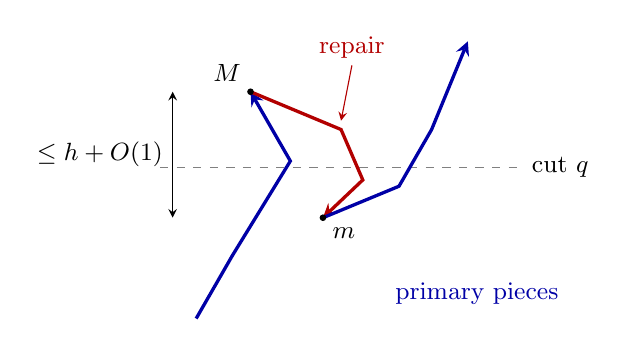
\begin{tikzpicture}[x=2.3cm,y=1.6cm,>=stealth,font=\small]
\draw[dashed,gray](-.2,1.2)--(1.8,1.2)
  node[right,black]{cut $q$};
\draw[very thick,blue!65!black,->]
  (0,0)--(.2,.5)--(.52,1.25)--(.3,1.8);
\draw[very thick,red!70!black,->]
  (.3,1.8)--(.8,1.5)--(.92,1.1)--(.7,.8);
\draw[very thick,blue!65!black,->]
  (.7,.8)--(1.12,1.05)--(1.3,1.5)--(1.5,2.2);
\fill(.3,1.8)circle(1.2pt) node[above left]{$M$};
\fill(.7,.8)circle(1.2pt) node[below right]{$m$};
\draw[<->](-.13,.8)--(-.13,1.8)
  node[midway,left]{$\le h+O(1)$};
\node[blue!65!black]at(1.55,.2){primary pieces};
\node[red!70!black]at(.86,2.15){repair};
\draw[red!70!black,thin,->](.86,2.01)--(.80,1.57);
\end{tikzpicture}
\caption{A repeated crossing of a transverse cut in an upward run.
The segment from the selected maximum $M$ to the following minimum $m$
is read downward; the neighboring pieces are read upward.  The drawing
is schematic and suppresses individual lattice edges.  The drawdown
bound controls the repair's height, while the separated cut levels keep
distinct repairs in ordered disjoint zones.}
\label{R:geo:repair-figure}
\end{figure}

Call the pieces in the original direction primary pieces.  Their spans
are between fixed positive multiples of $h$; repair spans are at most
$Ch$.  After the local port changes, test every turn with sufficiently
large smaller span.  If $P$ is the number of primary pieces, then
\begin{equation}\label{R:geo:primary-count}
                         c d/h\le P\le Cn/h.
\end{equation}
There are at most $P-1$ repairs, and the total modified length is at
most $n+CP$.

Apply Proposition~\ref{R:geo:chain} with $K=h^{3/4}$.  Write a
primary label as $\kappa_i=Kx_i$.  A repair of height scale $a\le Ch$
has $K_{\rm rep}=a^{3/4}$; put
$t=K_{\rm rep}/K$ and $y=\kappa_{\rm rep}/K\le t$.
Fixed comparability constants can be absorbed into all bounds below,
so the normalized labels are at most one.  For a single-crossing cut
without a repair use the formal values $a=K_{\rm rep}=\kappa_{\rm rep}=1$.
This virtual node has unit mass and no avoidance test; its algebraic
node and seam factors are also one, since every actual $\kappa_i\ge1$.

At either kind of cut, smooth the height of the preceding primary
piece.  Its endpoint lies within $O(a)$ of the cut, where the cut level
is specified relative to the run's starting height by the discrete cut
pattern.  We claim that this supplies the factor
\begin{equation}\label{R:geo:repair-smoothing}
                      C\min(1,(t/x_i)^{4/3}).
\end{equation}
Bounded-count nodes use the bounded-factor height estimate in
Proposition~\ref{R:geo:chain}.  At the other nodes, use this constraint
only when $a\kappa_i^{-4/3}<1$, and fix all coordinates outside the
selected reserved groups.  Their height sums
have a joint atom bound equal to the product of their individual bounds
$C\kappa_i^{-4/3}$ from Proposition~\ref{R:geo:chain}.  The allowed
height vectors can be counted in traversal order: once the earlier
selected sums in the run are given, the current endpoint constraint
allows at most $Ca$ values for the next sum.  The run's starting height
cancels from this relative constraint.  Thus the number of allowed
vectors is at most the product of these $Ca$ factors.  Multiplying by
the joint atom bound, and dropping the constraints at the unselected
nodes, proves the product of \eqref{R:geo:repair-smoothing}, since
$a\kappa_i^{-4/3}=(t/x_i)^{4/3}$.  Each primary receives at most one
factor.  This count already includes its possible endpoint heights.
The turn tests use only their separate history and rapid groups in
adjacent-port coordinates; none fixes the displacement of a selected
reserved group.

For completeness, the product calculation is as follows.  A direct
turn between primaries contributes $\max(x_i,x_{i+1})$ after the
primary factors have been collected.  A cut with a repair contributes
\[
 Q=\frac{\max(x_i,y)\max(x_{i+1},y)}{t}
                    \min(1,(t/x_i)^{4/3})
                 \le\max(x_{i+1},y).
\]
If $x_i\le t$, use $y\le t$; if $x_i>t$, the remaining factor is
$(t/x_i)^{1/3}\le1$.  This proves the inequality in both cases,
including the virtual-node convention.  The full product is bounded
by $Kx_1x_P$ times these factors and constant bases.  Every connecting
factor is bounded, and is $O(h^{-s})$ if all its incident labels are
less than $h^{-s}$.  The patterns of runs and cuts, repair scales,
count bins, and local records cost at most
$h^{C\eta(P+1)}$.

Take $s'=\epsilon/2$ and $s=9\epsilon/64$.  For small $\epsilon$
these choices satisfy $9s'/16>s$ and
\[
 \frac{n}{h^{4/3-s'}}=o\bigl(n^{3/4+\epsilon}/h\bigr).
\]
Set $l=h^{4/3-s'}$.  Since the total length is at most $n+CP$,
only $o(P)$ actual nodes have length greater than $l$.  Designate a
superset of these nodes; all possible designations cost at most
$2^{2P}$.  On every other actual node with normalized label at least
$h^{-s}$, the separate short-length group supplies
\[
 C e^{-c k_i q(l)}\le\exp(-h^{c_s}),
\]
for some $c_s>0$: indeed $k_i\ge K h^{-s}$ and
$K h^{-s}q(l)=h^{9s'/16-s+o(1)}$.  Virtual and bounded one-row
nodes have small labels.

If a positive fraction of labels are large, this gives stronger than
exponential decay in $P\log h$.  Otherwise a positive fraction of the
connections have all incident labels small.  Each large or designated
long node can spoil at most two such connections, so those connections
supply $h^{-s}$ each.  Choose $\eta$ sufficiently small after $s$.
After summing all the records and designations, the contribution with
$P$ primary pieces is at most $\exp(-cP\log h)$.  Equation
\eqref{R:geo:primary-count} gives the tall-bridge bound
\begin{equation}\label{R:geo:tall-bridge}
                  \exp(-c d\log h/h).
\end{equation}
All constants are uniform for $d$ in the stated range.

Finally take an unrestricted path of diameter at least $d$.  One of the
finitely many symmetry-related row normals has vertical span at least
$c d$.  In its extremum decomposition from
Proposition~\ref{R:geo:absolute-count}, an initial piece on one of
the two halves reaches the global maximum from the global minimum.
Omit that piece and its neighboring turn tests.  Its individual port
conversion has length at most $n+O(1)$ and height at least $c'd$;
its mass is bounded by \eqref{R:geo:tall-bridge}.  The remaining
pieces, including their choices and records, cost at most
$C_\delta e^{n^\delta}$ for every fixed $\delta>0$.
Choose $\delta$ smaller than the power gain in
$d/h\ge c n^{\epsilon+\gamma}$.  That cost is absorbed by
\eqref{R:geo:tall-bridge}.  This proves
\eqref{R:geo:fast-absolute}.  It also proves the uniform bound
\eqref{R:geo:fast-refined}, since $h\le n^{3/4}$ and the absorbed
exponent is a fixed fraction of $d\log h/h$.
\end{proof}
